\documentclass[10pt,border=4pt]{standalone}
\usepackage{mathptmx}
\usepackage{amsmath,amssymb,bm}
\usepackage{tikz}
\usetikzlibrary{patterns,decorations.pathmorphing,decorations.pathreplacing,arrows.meta,fit,backgrounds,calc,positioning,shapes.geometric}
\definecolor{acc}{HTML}{0B5394}
\definecolor{accl}{HTML}{EAF0F7}
\definecolor{grp}{HTML}{F5F5F5}
\definecolor{org}{HTML}{C55A11}
\definecolor{orgl}{HTML}{FBEFE6}
\tikzset{
 dat/.style={draw=black,line width=0.6pt,fill=white,align=center,font=\small,inner sep=3pt,minimum height=0.85cm},
 lay/.style={draw=acc,line width=0.8pt,fill=accl,rounded corners=2pt,align=center,font=\small,inner sep=3pt,minimum height=0.85cm},
 cnd/.style={draw=org,line width=0.8pt,fill=orgl,rounded corners=2pt,align=center,font=\small,inner sep=3pt,minimum height=0.75cm},
 op/.style={circle,draw=black,line width=0.6pt,fill=white,inner sep=0.5pt,font=\small,minimum size=5mm},
 grpb/.style={draw=black!45,dashed,line width=0.6pt,rounded corners=3pt,inner sep=6pt},
 arr/.style={-{Latex[length=2.2mm,width=1.7mm]},line width=0.7pt},
 carr/.style={-{Latex[length=2.2mm,width=1.7mm]},line width=0.7pt,draw=org},
 shp/.style={font=\scriptsize,text=black!70,inner sep=1pt},
 lab/.style={font=\footnotesize,inner sep=1pt},
 ttl/.style={font=\small\bfseries,inner sep=0pt,anchor=west}
}
\newcommand{\xh}{\mathbf{x}_h}\newcommand{\xf}{\mathbf{x}_f}

\begin{document}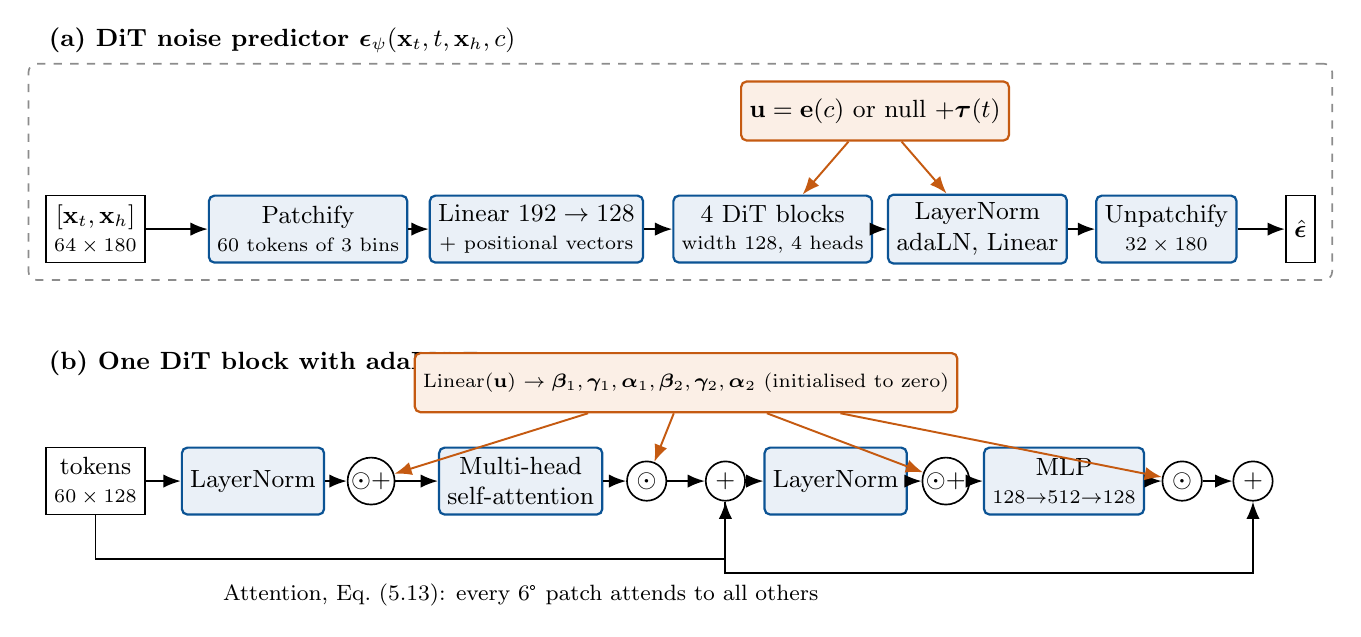
\begin{tikzpicture}[x=1cm,y=1cm]
\node[ttl] at (-0.6,2.4) {(a) DiT noise predictor $\boldsymbol\epsilon_\psi(\mathbf{x}_t,t,\xh,c)$};
\node[dat] (in) at (0,0) {$[\mathbf{x}_t,\xh]$\\[-1pt]\scriptsize $64\times180$};
\node[lay] (pat) at (2.7,0) {Patchify\\[-1pt]\scriptsize 60 tokens of 3 bins};
\node[lay] (emb) at (5.6,0) {Linear $192\to128$\\[-1pt]\scriptsize + positional vectors};
\node[lay] (blk) at (8.6,0) {4 DiT blocks\\[-1pt]\scriptsize width 128, 4 heads};
\node[lay] (fin) at (11.2,0) {LayerNorm\\adaLN, Linear};
\node[lay] (unp) at (13.6,0) {Unpatchify\\[-1pt]\scriptsize $32\times180$};
\node[dat] (eps) at (15.3,0) {$\hat{\boldsymbol\epsilon}$};
\draw[arr] (in)--(pat); \draw[arr] (pat)--(emb); \draw[arr] (emb)--(blk); \draw[arr] (blk)--(fin); \draw[arr] (fin)--(unp); \draw[arr] (unp)--(eps);
\node[cnd] (u) at (9.9,1.5) {$\mathbf{u}=\mathbf{e}(c)$ or null $+\boldsymbol\tau(t)$}; \draw[carr] (u)--(blk); \draw[carr] (u)--(fin);
\begin{scope}[on background layer]\node[grpb,fit=(in)(eps)(u)] {};\end{scope}
% (b) one block
\node[ttl] at (-0.6,-1.7) {(b) One DiT block with adaLN-Zero};
\node[dat] (h) at (0,-3.2) {tokens\\[-1pt]\scriptsize $60\times128$};
\node[lay] (ln1) at (2.0,-3.2) {LayerNorm};
\node[op] (m1) at (3.5,-3.2) {$\odot{+}$};
\node[lay] (att) at (5.4,-3.2) {Multi-head\\self-attention};
\node[op] (g1) at (7.0,-3.2) {$\odot$};
\node[op] (a1) at (8.0,-3.2) {$+$};
\node[lay] (ln2) at (9.4,-3.2) {LayerNorm};
\node[op] (m2) at (10.8,-3.2) {$\odot{+}$};
\node[lay] (mlp) at (12.3,-3.2) {MLP\\[-1pt]\scriptsize $128{\to}512{\to}128$};
\node[op] (g2) at (13.8,-3.2) {$\odot$};
\node[op] (a2) at (14.7,-3.2) {$+$};
\draw[arr] (h)--(ln1); \draw[arr] (ln1)--(m1); \draw[arr] (m1)--(att); \draw[arr] (att)--(g1); \draw[arr] (g1)--(a1); \draw[arr] (a1)--(ln2); \draw[arr] (ln2)--(m2); \draw[arr] (m2)--(mlp); \draw[arr] (mlp)--(g2); \draw[arr] (g2)--(a2);
\draw[arr] (h.south) -- ++(0,-0.55) -| (a1.south); \draw[arr] (8.0,-3.2) ++(0,-0.27) -- ++(0,-0.9) -| (a2.south);
\node[cnd] (ada) at (7.5,-1.95) {\scriptsize Linear($\mathbf{u}$) $\to\boldsymbol\beta_1,\boldsymbol\gamma_1,\boldsymbol\alpha_1,\boldsymbol\beta_2,\boldsymbol\gamma_2,\boldsymbol\alpha_2$ (initialised to zero)};
\foreach \n in {m1,g1,m2,g2} \draw[carr] (ada) -- (\n);
\node[lab] at (5.4,-4.65) {Attention, Eq.~(5.13): every 6° patch attends to all others};
\end{tikzpicture}\end{document}
